% !TeX root = main.tex
%%%%%%%%%%%%%%%%%%%%%%%%% PREAMBLE %%%%%%%%%%%%%%%%%%%%%%%%%%%%%%%%
%%%%%%%%%%%%%%%%%%%%%%%% BASIC DOCUMENT SETUP %%%%%%%%%%%%%%%%%%%%%
\documentclass[a4paper]{report}
\usepackage[utf8]{inputenc}
\usepackage[english]{babel}

%%%%%%%%%%%%%%%%%%%%%%%%%% PACKAGES %%%%%%%%%%%%%%%%%%%%%%%%%%%%%%%
\usepackage{datetime}
\usepackage{datenumber}
\usepackage{parskip}
\usepackage{forest}
\usepackage{svg}        % makes it possible to use svg files
\usepackage{graphics}
\usepackage{multicol}
\usepackage{icomma}
\usepackage{microtype}  % microscopic typography refinement
\usepackage{lastpage}   % used to reference last page in footer
\usepackage{fancyhdr}   % Header
\usepackage{tcolorbox}
\usepackage{amssymb}
\usepackage[Bjornstrup]{fncychap}
\usepackage[titles]{tocloft}
\usepackage{amsmath}    % mathematics for matrices and more
\usepackage{amsfonts}
\usepackage{csquotes}
\usepackage{morewrites}

\usepackage{tikz}
\usetikzlibrary{calc}   % position og tikz labels
\usetikzlibrary{arrows.meta}
\usetikzlibrary{decorations.pathreplacing,calligraphy}

\usepackage{float}
\usepackage{pgfplots}
\pgfplotsset{compat=1.17}
\usepackage{xcolor}
\definecolor{blueplot}{RGB}{60, 64, 198}
\definecolor{yellowplot}{RGB}{255, 211, 42}
\definecolor{redplot}{RGB}{255, 63, 52}
\definecolor{greenplot}{RGB}{5, 196, 107}
\definecolor{greyplot}{RGB}{72, 84, 96}

\usepackage{siunitx}
\sisetup{%quotient-mode=fraction,
		output-decimal-marker = {,},
		per-mode = fraction,
		separate-uncertainty = true,
		multi-part-units=single,
		exponent-product = \cdot,
		range-phrase=--}
		
\usepackage{minted} % Syntax highlighting 
%\usemintedstyle{monokai}
\setminted[]{breaklines, 
    breakafter=d,
    frame=lines,
    framesep=2mm,
    baselinestretch=1.2,
    fontsize=\footnotesize,
    tabsize=4,
    linenos}


\makeatletter
\renewcommand\@makefnmark{\textsuperscript{[\@thefnmark]}}
\renewcommand\@makefntext[1]{\textsuperscript{[\@thefnmark]}\enspace #1}
\makeatother

\usepackage[hidelinks, linktoc=all]{hyperref} % links, references, \ref{...}
\hypersetup{
    colorlinks = true,
    linkcolor = blue,
    citecolor = blue,
    urlcolor = blue
}
\urlstyle{same}

\usepackage{todonotes}

\usepackage{subcaption}

\usepackage{forest}

\usepackage{lipsum}  

\usepackage{misc/quiver}

\usepackage{wrapfig}

\usepackage[export]{adjustbox}


\usepackage[pdf]{graphviz}

%%% Helper code for Overleaf's build system to
%%% automatically update output drawings when
%%% code in a \digraph{...} is modified
\usepackage{xpatch}
\makeatletter
\newcommand*{\addFileDependency}[1]{% argument=file name and extension
  \typeout{(#1)}
  \@addtofilelist{#1}
  \IfFileExists{#1}{}{\typeout{No file #1.}}
}
\makeatother
\xpretocmd{\digraph}{\addFileDependency{#2.dot}}{}{}

\usepackage[block=ragged, sorting=nyt, style=authoryear-ibid, backend=biber]{biblatex}
\setlength\bibitemsep{1.5\itemsep}
\addbibresource{misc/mybib.bib}

%%%%%%%%%%%%% ACTUAL VISIBLE CONTENT %%%%%%%%%%%%%%%%%%%%%%%%%%%%%%
\begin{document}
\begin{titlepage}
\begin{centering}
\vspace*{-20px}\large Department of Mathematics \& Computer Science\\
University of Southern Denmark $|$ IMADA \\
\today \\

\vspace{4CM}

\huge{\bf  Compiler for Panda} \\
\Large{\bf BADM500: Bachelor Project}

\vspace{\fill}

\begin{minipage}{0.45\textwidth} 
\begin{flushleft}
    \Large
    \textit{Author}\\
    KIAN BANKE LARSEN\\
    kilar20@student.sdu.dk
\end{flushleft}
\end{minipage}

\vspace{\fill}

\begin{minipage}{0.45\textwidth}
\begin{flushleft}
    \Large
    \textit{Supervisor}\\
    KIM SKAK LARSEN\\
    Professor
\end{flushleft}
\end{minipage}

\vspace{\fill}

\includesvg[width=.4\textwidth]{misc/SDU.svg}\vspace*{-0.95cm}

\end{centering}

\thispagestyle{empty}
\end{titlepage}

\pagenumbering{roman}

\begin{abstract}
    \paragraph{English}
    This is my very good abstract

    \paragraph{Danish}
    Et fantastisk abstract
\end{abstract}

{ \hypersetup{hidelinks} \tableofcontents }

\newpage
\pagenumbering{arabic}
\setcounter{page}{1}

\chapter{Introduction}
This report examines how to make a simple compiler in Python. The compiler is simple in the sense that some decisions have been made to ease the process, despite the choice, although the decisions are not necessarily optimal. The aim is to learn different compiler techniques and get a hands-on feel for the different compiler phases by actually implementing a working compiler, targeting X86 assembler, from scratch, using a Flex/Bison equivalent package such as \texttt{PLY} for scanning and parsing. 

The language to be compiled is a subset of the imperative language C. This has been chosen because of its simpler syntax and easy to read curly bracket enclosed static scopes. In this project, we are interested in making a language having integers, Booleans and preferably some kind of floats. The language must have control flow constructs in form of \texttt{if}-\texttt{else} statements and functions, and iterative constructs such as \texttt{for}- and \texttt{while}-loops. 

A modern compiler is, as is well known, divided into phases. These phases relate to lexical and syntactic analysis, resulting in an abstract syntax tree. Subsequent phases analyze and adorn the abstract syntax tree, building a symbol table and finally generating assembler code.

The main focus in regard to advanced techniques will be local register allocation, using techniques described in \cite{EnginneringACompiler}. Handling this efficiently requires data flow analysis via control flow-graph, construction of interference graph, graph coloring and translation back to instructions using a combination of the registers and the stack, when the available registers do not suffice.

Initially, a stack machine will be prepared, which will form the basis for developing a compiler that uses CPU registers. We will take advantage of the split phases property when replacing the stack code generation phase in benefit for one that uses register allocation. This allows us to only worry about ensuring that subsequent phases cope with the changes made in the former phases.

When adding extra complexity such as register allocation, it is important to document the benefit of this choice. Performance of the stack machine and the register machine will therefore be constructively compared.

\chapter{Project Basics}
This section is reserved for articulating some choices made at the very beginning of the project that defined the framework for how to develop and use the compiler.

\section{Project Structure}
The Compiler module uses different python packages -- things that belong together must be together. It has been desired to make a clear division between the different phases, and this has been achieved by creating the Python package \texttt{phase}. Likewise, \texttt{dataclass} is a package that contains internal data structures, in other words, classes used to hold data. \texttt{Printer} is a package that is used primarily for debugging, but sometimes it is just nice to consider data structures graphically. \texttt{Testing} is placed on the same level as \texttt{src} because it has nothing to do with the compiler's implementation, it is just a QA tool that makes it easier to verify correctness. \texttt{compiler.py} takes care of summarizing all functionality, but the module requires arguments from the command line, and those arguments (as well as testing) are handled in \texttt{main.py}, which is why \texttt{main.py} can be considered the project's main file.
\begin{figure}[H]
    \centering
    \begin{subfigure}{0.3\textwidth}
    \centering
    \scalebox{0.65}{
\begin{forest}
  for tree={
    font=\ttfamily,
    grow'=0,
    child anchor=west,
    parent anchor=south,
    anchor=west,
    calign=first,
    edge path={
      \noexpand\path [draw, \forestoption{edge}]
      (!u.south west) +(7.5pt,0) |- node[fill,inner sep=1.25pt] {} (.child anchor)\forestoption{edge label};
    },
    before typesetting nodes={
      if n=1
        {insert before={[,phantom]}}
        {}
    },
    fit=band,
    before computing xy={l=15pt},
  }
[Compiler/
    [src/
        [dataclass/
            [AST.py]
            [iloc.py]
            [symbol.py]
        ]
        [printer/
            [ast\_printer.py]
            [generic\_printer.py]
            [symbol\_printer.py]
        ]
    ]
]
\end{forest}
}
    \end{subfigure}        
    \hfill
    \begin{subfigure}{0.3\textwidth}
    \centering
    \scalebox{0.7}{
\begin{forest}
  for tree={
    font=\ttfamily,
    grow'=0,
    child anchor=west,
    parent anchor=south,
    anchor=west,
    calign=first,
    edge path={
      \noexpand\path [draw, \forestoption{edge}]
      (!u.south west) +(7.5pt,0) |- node[fill,inner sep=1.25pt] {} (.child anchor)\forestoption{edge label};
    },
    before typesetting nodes={
      if n=1
        {insert before={[,phantom]}}
        {}
    },
    fit=band,
    before computing xy={l=15pt},
  }
[Compiler/
    [src/
        [printer/
            [ast\_printer.py]
            [generic\_printer.py]
            [symbol\_printer.py]
        ]
        [utils/]
        [compiler.py]
    ]
    [testing/
        [test-cases/]
        [test.py]
    ]
    [main.py]
    [README.md]
    [...]
]
\end{forest}
}
    \end{subfigure}
    \hfill
    \begin{subfigure}{0.3\textwidth}
    \centering
    \scalebox{0.65}{
\begin{forest}
  for tree={
    font=\ttfamily,
    grow'=0,
    child anchor=west,
    parent anchor=south,
    anchor=west,
    calign=first,
    edge path={
      \noexpand\path [draw, \forestoption{edge}]
      (!u.south west) +(7.5pt,0) |- node[fill,inner sep=1.25pt] {} (.child anchor)\forestoption{edge label};
    },
    before typesetting nodes={
      if n=1
        {insert before={[,phantom]}}
        {}
    },
    fit=band,
    before computing xy={l=15pt},
  }
[Compiler/
    [src/
        [utils/]
        [compiler.py]
    ]
    [testing/
        [test-cases/]
        [test.py]
    ]
    [main.py]
    [README.md]
    [...]
]
\end{forest}
}
    \end{subfigure}
    \caption{Project file tree.}
\end{figure}

\section{Python Lex-Yacc}
PLY is a native Python tool, relying on reflection, used to automatically generate scanners and LALR(1) parsers. The package is well documented at the following source: \cite{ply}. Usage of the package will be described when reviewing the compiler phases in isolation. It has been chosen to use PLY in order to reserve more time for the compiler itself, though studies show that most compilers use hand-coded scanners \parencite[69]{EnginneringACompiler}. However, tool-generated parsers are more common than handed-parsers \parencite[85]{EnginneringACompiler}.

\section{Design Principles \& Patterns}
When starting a new project, it is important to make some basic thoughts about the architecture. Sensible choices at the beginning can increase code readability and make maintainability easier. It is particularly important to consider design principles and design patterns, as this will have a big effect on, i.e., how data structures are traversed and code testability. In this context, design principles refer to SOLID, and design patterns refer to Gang of Four's 23 design patterns.

We will start by considering design principles. SOLID is a mnemonic acronym for at set of design principles concerning software development in object-oriented languages: \textbf{S}ingle Responsibility, \textbf{O}pen Closed, \textbf{L}iskov's Substitution, \textbf{I}nterface Segregation and \textbf{D}ependency Inversion. The principles are in many ways obvious when rehearsed, but not necessarily followed as it requires active consideration. Single responsibility is particularly expressed in the project by the sharp division of phases and their interfaces between them. Open/closed is not particularly used in the project, as inheritance cases sparsely appear, though crucial in the printer package. It will never be necessary to edit the generic printer because functionality to print a specific data structure is first implemented upon extension. Liskov's substitution principle is accommodated in the AST data class, since any subtree is a valid tree and all nodes are AST nodes. Dependency inversion principle simply means that you must program against an interface and not an implementation. There is actually an incident where the project does not live up to this principle, and that is when using the hidden method \texttt{\_value2member\_map\_} on \texttt{Enum} in the parsing phase. Other examples apply, of course, as every class must accommodate every principle. This was just a quick review.

One of the big decisions regarding behavioral design patterns has been whether to use Visitors, just like in the well known SCIL compiler from the DM565 course. It was decided not to use visitors, because Python 3.10 comes with a new cool feature, namely match statements, which makes it possible to exploit the benefits of structural pattern matching. Although it is nice to let the data structure decide its iteration, I still prefer having everything written explicitly when learning to write a compiler. Using match statements requires one to repeat the iteration logic for every new operation, but that kind of also makes it easier to implement new logic, as one does not have to remember the visitor pattern. Another useful creational design pattern is the Singleton pattern used in \texttt{label\_generator.py}. This makes it possible to retrieve the label generator in any class, while preserving the state on \texttt{count}, without having to pass the object through all the phases manually.

\section{Compiler Usage}
The main file handles the instantiation and therefore also the running of the \texttt{PandaCompiler} class. Python \texttt{argparse} is used to take command line arguments. Python \texttt{argparse} adds a lot of user-friendliness to the compiler, because one get the opportunity to query the use of the compiler in the terminal, thus see what options are available. Doing so yields the result stated below:

\begin{minted}{text}
Compiler$ python3.10 main.py --help

usage: Compiler for Panda [-h] [-o OUTPUT] [-c] [-d] [-f FILE] [-t] [-r]

Compiles source code to assembly

options:
    -h, --help            show this help message and exit
    -o OUTPUT, --output OUTPUT
                        Specify name of assembly output file
    -c, --compile         Set this flag if the output file should be compilled with gcc
    -d, --debug           Set this flag for debugging information, i.e., ILOC and Graphviz
    -f FILE, --file FILE  Path to input file, otherwise stdin will be used
    -t, --runTests        Run tests
    -r, --run             Run compilled program
\end{minted}

This informs the user that one can specify an input file or provide input directly in the command line, and specifying the name of the output file is optional. Furthermore, one can control whether the file should be automatically compiled with \texttt{gcc} and directly run on the system. Many of the arguments act as flags to the compiler, such as \texttt{--debug} or \texttt{--runTests}, which are flags that specify whether a certain piece of code should be executed. Much of the setup of \texttt{argparse} is omitted, in this example, but the essential part of the functionality is listed below. All pip requirements needed for running \texttt{main.py} can be installed using \texttt{pip install -r requirements.txt} -- file located in the root of the project.

\begin{minted}{py3}
args = argparser.parse_args()

if args.runTests:
    runner = unittest.TextTestRunner(verbosity=2)
    result = runner.run(testing.test.load_tests(args))
else:
    PandaCompiler(args).compile()
\end{minted}

If the \texttt{--runTests} flag is set, then it will take priority over the regular compiler functionality. However, it is still possible to specify \texttt{--debug}, as debugging information may be useful in case some tests fail. Debugging information is information such as graphical representation of data structures and pretty printed ILOC code -- sequential assembly IR. Testing will be explained in depth later.

\chapter{Phases}
\section{Lexical Analysis}
\newpage
\section{Parsing}
\begin{figure}[H]
    \centering
    \digraph[scale=0.5]{ast}{
	0 [label="?main"]
	1 [label=body]
	2 [label=init_var_decl]
	3 [label=5]
	4 [label=int]
	5 [label=j]
	2 -> 4
	2 -> 5
	2 -> 3
	6 [label=decl_list]
	6 -> 2
	1 -> 6
	7 [label=stm_list]
	8 [label=init_var_decl]
	9 [label=1]
	10 [label=int]
	11 [label=i]
	8 -> 10
	8 -> 11
	8 -> 9
	12 [label=i]
	13 [label=5]
	14 [label="<"]
	14 -> 12
	14 -> 13
	15 [label=i]
	16 [label=1]
	17 [label="+"]
	17 -> 15
	17 -> 16
	18 [label="="]
	19 [label=i]
	18 -> 19
	18 -> 17
	20 [label=body]
	21 [label=for]
	21 -> 8
	21 -> 14
	21 -> 18
	21 -> 20
	7 -> 21
	1 -> 7
	0 -> 1
}

    \caption{Abstract Syntax Tree.} 
\end{figure}
\newpage
\section{Symbol Collection}
\begin{figure}[H]
    \centering
    \digraph[scale=0.5]{symbol}{
	graph [rankdir=BT]
	0 [label=j]
	1 [label=i]
	1 -> 0
}

    \caption{Symbol collection.} 
\end{figure}
\newpage
\section{Desugaring}
\begin{figure}[H]
    \centering
    \digraph[scale=0.37]{desugar}{
	0 [label="?main"]
	1 [label=body]
	2 [label=init_var_decl]
	3 [label=5]
	4 [label=int]
	5 [label=j]
	2 -> 4
	2 -> 5
	2 -> 3
	6 [label=decl_list]
	6 -> 2
	1 -> 6
	7 [label=stm_list color="black" fillcolor="yellow" style=filled]
	8 [label=5 color="black" fillcolor="yellow" style=filled]
	9 [label="=" color="black" fillcolor="yellow" style=filled]
	10 [label=j color="black" fillcolor="yellow" style=filled]
	9 -> 10
	9 -> 8
	7 -> 9
	11 [label=stm_list]
	12 [label=init_var_decl]
	13 [label=1]
	14 [label=int]
	15 [label=i]
	12 -> 14
	12 -> 15
	12 -> 13
	16 [label=i]
	17 [label=5]
	18 [label="<"]
	18 -> 16
	18 -> 17
	19 [label=i]
	20 [label=1]
	21 [label="+"]
	21 -> 19
	21 -> 20
	22 [label="="]
	23 [label=i]
	22 -> 23
	22 -> 21
	24 [label=body]
	25 [label=for]
	25 -> 12
	25 -> 18
	25 -> 22
	25 -> 24
	11 -> 25
	7 -> 11
	1 -> 7
	0 -> 1
}

    \caption{Desugaring tree.} 
\end{figure}
\newpage
\section{Code Generation} 
\subsection{Stack Machine}
\subsection{Register Allocation}

\chapter{Testing}
The main benefit of testing is the identification and subsequent mitigation of errors. It is to be expected to find errors in larger projects, which is why there must be a way to quickly and dynamically run tests during development. Testing helps software developers compare expected and actual output in order to improve quality. In this case, only system testing is carried out, although a higher granularity of testing would only enrich the project. There exist many tools to solve this task, which is why the big challenge lies in choosing the one that best suits the problem. The most advanced tool is not always the best solution. The chosen tools in this project are the testing framework \texttt{unittest} and the coverage tool \texttt{coverage.py}. In addition, SonarLint is used to perform static code analysis within the IDE to provide best-practice hints, cognitive complexity metrics and more -- not important but worth mentioning.

\section{System Testing}
The most common choice would have been to use \texttt{pytest} because it is significantly more popular than \texttt{unittest}, but for the task \texttt{unittest} seemed like the right choice. I am not able to judge whether the same could have been achieved using \texttt{pytest} with parametrized tests, but setting up \texttt{unittest} was straight forward.

I wanted a solution where it is possible to load tests dynamically, based on test files in a given folder. Hence, it would not be necessary to write more code just because tests are added to the test suite -- writing test cases must not be a burden; otherwise it will not be done. The idea is as follows (in pseudo Python):

\begin{minted}{py3}
class TestCase(unittest.TestCase):
    def __init__(self, <args>) -> TestCase:
        super().__init__()

        def runTest(self):
            pass
\end{minted}

First, A class inheriting from \texttt{unittest.TestCase} is declared, which makes it possible to define a test case with the required interface. A single test case can then be created by creating an instance of \texttt{TestCase}. A test case is created for every pair of \texttt{file.panda} and \texttt{file.eop} by walking the directory \texttt{test-cases}.

\begin{minted}{py3}
def load_tests(args: argparse.Namespace) -> unittest.TestSuite:
    test_cases = unittest.TestSuite()

    for src, res in test-cases:
        test_cases.addTest(TestCase(src, res))
\end{minted}

The method named \texttt{runTest} will be executed when running the test, unless otherwise specified. \texttt{runTest} has the responsibility to report whether an individual test succeeds or fails. My \texttt{runTest} does the following:

\begin{enumerate}
    \item Compile source code;
    \item Execute compiled code and pipe \texttt{std:out} to file;
    \item Assert whether output and expected output is identical.
\end{enumerate}

Of course, some exception handling needs to be done, but that is the basics. An interesting necessary exception handling is when running a test developed to fail, as the exception handling in the compiler will execute \texttt{os.exit(1)} (it does not make sense to continue), so that exception must be caught in the running test in order to retrieve whatever is printed to \texttt{std:err}.

The test suite can be run as follows when the desired tests have been added:

\begin{minted}{py3}
runner = unittest.TextTestRunner(verbosity=2)
result = runner.run(testing.test.load_tests(args))
\end{minted}

The above logic is contained within \texttt{main.py} and wrapped in an \texttt{if-else} statement. Running the tests therefore requires calling main.py with option \texttt{--runTests} or simply \texttt{-t}, as shown below:

\begin{minted}{text}
Compiler$ python3.10 main.py --runTests

runTest (testing.test.TestCase)
Testing testing/test-cases/fibonacci_classic.panda ... ok
runTest (testing.test.TestCase)
Testing testing/test-cases/static_nested_scope.panda ... ok
...
----------------------------------------------------------------------
Ran 21 tests in 2.261s

OK 
\end{minted}

The test suite is automatically run on every pull request or push to GitHub as part of the CI workflow using GitHub Actions. Configuration can be found in \texttt{/.github/workflows/unittest.yml}.

\section{Coverage}
\begin{minted}{text}
Compiler$ python3.10 -m coverage run main.py --runTests -d

Name                                     Stmts   Miss  Cover
------------------------------------------------------------
main.py                                     21      1    95%
src/compiler.py                             59      3    95%
src/dataclass/AST.py                       125      0   100%
src/dataclass/iloc.py                       22      0   100%
src/dataclass/symbol.py                     35      2    94%
src/enums/code_generation_enum.py           39      0   100%
src/enums/symbols_enum.py                    5      0   100%
src/phase/code_generation_base.py           57      3    95%
src/phase/code_generation_register.py      232      8    97%
src/phase/code_generation_stack.py         196      3    98%
src/phase/emit.py                          128      6    95%
src/phase/lexer.py                          44      8    82%
src/phase/parser.py                        101      3    97%
src/phase/parsetab.py                       18      0   100%
src/phase/symbol_collection.py              86      0   100%
src/phase/syntactic_desugaring.py           65      0   100%
src/printer/ast_printer.py                 141      3    98%
src/printer/generic_printer.py              17      0   100%
src/printer/symbol_printer.py               40      0   100%
src/utils/error.py                           5      0   100%
src/utils/interfacing_parser.py              1      0   100%
src/utils/label_generator.py                 9      0   100%
src/utils/x86_instruction_enum_dict.py       2      0   100%
testing/test.py                             73      0   100%
... 
... 
...
...
------------------------------------------------------------
TOTAL                                     1521     40    97%
Wrote HTML report to htmlcov/index.html
\end{minted}

\begin{figure}[H]
    \centering
    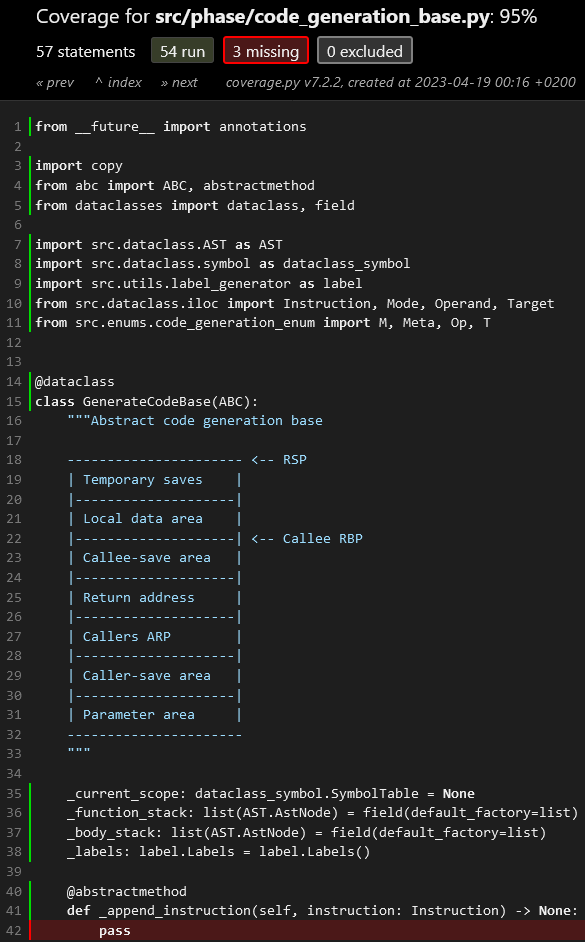
\includegraphics[width=.9\textwidth]{misc/images/coverage_full.png}
    \caption{Coverage HTML report.}
\end{figure}


\chapter{Performance Comparison}

\chapter{Evaluation}
\section{Language Considerations}
\section{Further Development}
 
\chapter{Conclusion}

\cleardoublepage
\phantomsection
\addcontentsline{toc}{chapter}{References}
\printbibliography
\end{document}